\chapter{Les différents équipements}\label{devices}
\section{Le HIL DSpace}
Continental possède différentes tables de tests avec des simulateurs d'environnement véhicule DSPace, comme montré figure \ref{fig:dspace}.
\begin{figure}[H]
	\centering
	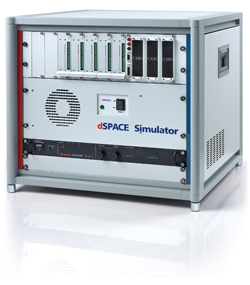
\includegraphics[width=8cm]{contents/images/hil.jpg}
	\caption{HIL DSpace}
	\label{fig:dspace}
\end{figure}

Ce simulateur peut être contrôlé via un ordinateur et le logiciel \textit{ControlDesk}. Ce logiciel permet de pouvoir modifier tous les
paramètres souhaités de la voiture, comme la tension, la vitesse de rotation du moteur, la mise en place du starter, \ldots

Une capture d'écran de cette interface est disponible figure \ref{fig:controldesk}.

\begin{figure}[H]
	\centering
	% TODO TODO TODO
%	\includegraphics[width=8cm]{contents/images/tlp.jpg}
	\caption{HIL DSpace}
	\label{fig:controldesk}
\end{figure}

\section{Le Debugger}
L'entreprise possède des Debuggers permettant de flasher le programme sur le calculateur, de lire l'état des variables, de modifier des
variables, des calibrations, \ldots

Ce contrôle peut se faire via le logiciel \textit{TLPcasso} dont une capture d'écran est présenté figure \ref{fig:tlp}. TLP permet d'appeler
toute sortes de scripts afin d'effectuer simplement certaines actions.

\begin{figure}[H]
	\centering
	% TODO TODO TODO
%	\includegraphics[width=8cm]{contents/images/tlp.jpg}
	\caption{HIL DSpace}
	\label{fig:tlp}
\end{figure}
